\pdfminorversion=4
\documentclass{beamer}

\usepackage[toc]{beamerthemecea2019}
\usepackage[T1]{fontenc}
\usepackage[utf8]{inputenc}

\usepackage{longtable}
%\usepackage{couleurs}
\usepackage{listings}
%\usepackage{mecanique}
\usepackage{pifont}% http://ctan.org/pkg/pifont
\usepackage{animate,subcaption}
\usepackage[absolute,overlay]{textpos}
\setlength{\TPHorizModule}{\paperwidth}
\setlength{\TPVertModule}{\paperheight}

\newcommand{\backupbegin}{
   \newcounter{finalframe}
   \setcounter{finalframe}{\value{framenumber}}
}
\newcommand{\backupend}{
   \setcounter{framenumber}{\value{finalframe}}
}
\setbeamercolor{block title}{bg=cea_rouge!90,fg=white}
\newcommand{\dx}{\text{ dx}}
\newcommand{\dS}{\text{ dS}}
\newcommand{\udl}[1]{\boldsymbol{#1}}
\newcommand{\uddl}[1]{\boldsymbol{#1}}
\renewcommand{\div}{\operatorname{div}}
\newcommand{\bg}{\boldsymbol{g}}
\newcommand{\bj}{\boldsymbol{j}}
\newcommand{\bu}{\boldsymbol{u}}
\newcommand{\bv}{\boldsymbol{v}}
\newcommand{\bvarepsilon}{\boldsymbol{\varepsilon}}
\newcommand{\bsig}{\boldsymbol{\sigma}}
\newcommand{\bD}{\boldsymbol{D}}
\newcommand{\bE}{\boldsymbol{E}}
\newcommand{\bF}{\boldsymbol{F}}
\newcommand{\bR}{\boldsymbol{R}}
\newcommand{\bH}{\boldsymbol{H}}
\newcommand{\bI}{\boldsymbol{I}}
\newcommand{\bP}{\boldsymbol{P}}
\newcommand{\bS}{\boldsymbol{S}}
\newcommand{\bT}{\boldsymbol{T}}
\newcommand{\bV}{\boldsymbol{V}}
\newcommand{\bY}{\boldsymbol{Y}}
\newcommand{\Bb}{\mathcal{B}}
\newcommand{\Dd}{\mathcal{D}}
\newcommand{\Ee}{\mathcal{E}}
\newcommand{\CC}{\mathbb{C}}
\newcommand{\DD}{\mathbb{D}}
\newcommand{\TT}{\mathbb{T}}
\newcommand{\Sig}{\boldsymbol{\Sigma}}
\newcommand{\T}{^\text{T}}
\newcommand{\jump}[1]{[\![#1]\!]}
\DeclareMathOperator*{\argmin}{arg\,min}
\DeclareMathOperator{\tr}{tr}
\newcommand{\pavg}[1]{\left\langle #1 \right\rangle}

\newcommand{\Cxx}{\texttt{C\nolinebreak\hspace{-.05em}\raisebox{.4ex}{\tiny\bf +}\nolinebreak\hspace{-.10em}\raisebox{.4ex}{\tiny\bf +}}
  \def\CC{{C\nolinebreak[4]\hspace{-.05em}\raisebox{.4ex}{\tiny\bf ++}}}}
\newcommand{\tfel}{\href{http://www.tfel.sourceforge.net}{\texttt{TFEL}}}
\newcommand{\mfront}{\href{http://www.tfel.sourceforge.net}{\texttt{MFront}}}
\newcommand{\cea}{\href{http://www.cea.fr}{CEA}}
\newcommand{\edf}{\href{http://www.edf.com}{EDF}}
\newcommand{\inria}{\href{http://www.inria.fr}{INRIA}}
\newcommand{\gcc}{\href{https://gcc.gnu.org/}{gcc}}
\newcommand{\clang}{\href{clang.llvm.org}{clang}}
\newcommand{\icc}{\href{https://software.intel.com/en-us/c-compilers}{icc}}
\newcommand{\msys}{\href{http://www.mingw.org/wiki/MSYS}{MSYS}}
\newcommand{\jenkins}{\href{http://jenkins-ci.org}{\texttt{Jenkins}}}
\newcommand{\gpl}{\href{http://www.gnu.org/licenses/gpl-3.0.txt}{GNU Public License}}
\newcommand{\unix}{\texttt{Unix}}
\newcommand{\linux}{\texttt{LiNuX}}
\newcommand{\freebsd}{\href{https://www.freebsd.org/}{\texttt{FreeBSD}}}
\newcommand{\opensolaris}{\texttt{OpenSolaris}}
\newcommand{\cygwin}{\texttt{cygwin}}
\newcommand{\wsl}{\texttt{Windows Subsystem for LiNuX}}
\newcommand{\haiku}{\texttt{Haiku}}
\newcommand{\mtest}{\texttt{mtest}}
\newcommand{\absvalue}[1]{{\left|#1\right|}}

\usepackage{fancyvrb}
\newcommand{\VerbBar}{|}
\newcommand{\VERB}{\Verb[commandchars=\\\{\}]}
\DefineVerbatimEnvironment{Highlighting}{Verbatim}{commandchars=\\\{\}}
\newenvironment{Shaded}{}{}
\newcommand{\AlertTok}[1]{\textcolor[rgb]{1.00,0.00,0.00}{\textbf{#1}}}
\newcommand{\AnnotationTok}[1]{\textcolor[rgb]{0.38,0.63,0.69}{\textbf{\textit{#1}}}}
\newcommand{\AttributeTok}[1]{\textcolor[rgb]{0.49,0.56,0.16}{#1}}
\newcommand{\BaseNTok}[1]{\textcolor[rgb]{0.25,0.63,0.44}{#1}}
\newcommand{\BuiltInTok}[1]{#1}
\newcommand{\CharTok}[1]{\textcolor[rgb]{0.25,0.44,0.63}{#1}}
\newcommand{\CommentTok}[1]{\textcolor[rgb]{0.38,0.63,0.69}{\textit{#1}}}
\newcommand{\CommentVarTok}[1]{\textcolor[rgb]{0.38,0.63,0.69}{\textbf{\textit{#1}}}}
\newcommand{\ConstantTok}[1]{\textcolor[rgb]{0.53,0.00,0.00}{#1}}
\newcommand{\ControlFlowTok}[1]{\textcolor[rgb]{0.00,0.44,0.13}{\textbf{#1}}}
\newcommand{\DataTypeTok}[1]{\textcolor[rgb]{0.56,0.13,0.00}{#1}}
\newcommand{\DecValTok}[1]{\textcolor[rgb]{0.25,0.63,0.44}{#1}}
\newcommand{\DocumentationTok}[1]{\textcolor[rgb]{0.73,0.13,0.13}{\textit{#1}}}
\newcommand{\ErrorTok}[1]{\textcolor[rgb]{1.00,0.00,0.00}{\textbf{#1}}}
\newcommand{\ExtensionTok}[1]{#1}
\newcommand{\FloatTok}[1]{\textcolor[rgb]{0.25,0.63,0.44}{#1}}
\newcommand{\FunctionTok}[1]{\textcolor[rgb]{0.02,0.16,0.49}{#1}}
\newcommand{\ImportTok}[1]{#1}
\newcommand{\InformationTok}[1]{\textcolor[rgb]{0.38,0.63,0.69}{\textbf{\textit{#1}}}}
\newcommand{\KeywordTok}[1]{\textcolor[rgb]{0.00,0.44,0.13}{\textbf{#1}}}
\newcommand{\NormalTok}[1]{#1}
\newcommand{\OperatorTok}[1]{\textcolor[rgb]{0.40,0.40,0.40}{#1}}
\newcommand{\OtherTok}[1]{\textcolor[rgb]{0.00,0.44,0.13}{#1}}
\newcommand{\PreprocessorTok}[1]{\textcolor[rgb]{0.74,0.48,0.00}{#1}}
\newcommand{\RegionMarkerTok}[1]{#1}
\newcommand{\SpecialCharTok}[1]{\textcolor[rgb]{0.25,0.44,0.63}{#1}}
\newcommand{\SpecialStringTok}[1]{\textcolor[rgb]{0.73,0.40,0.53}{#1}}
\newcommand{\StringTok}[1]{\textcolor[rgb]{0.25,0.44,0.63}{#1}}
\newcommand{\VariableTok}[1]{\textcolor[rgb]{0.10,0.09,0.49}{#1}}
\newcommand{\VerbatimStringTok}[1]{\textcolor[rgb]{0.25,0.44,0.63}{#1}}
\newcommand{\WarningTok}[1]{\textcolor[rgb]{0.38,0.63,0.69}{\textbf{\textit{#1}}}}

% orange
\definecolor{lightorange}{rgb}{1.0,0.63921,0.3961}
\definecolor{orange}{rgb}{1.0,0.5098, 0}

% chocolate (brownish)
\definecolor{my_blue}{rgb}{0.09019,0.4706,1.0}
\definecolor{lightblue}{rgb}{0.8588,0.9490,1.0}


\newcommand{\cmark}{\textcolor{green}{\ding{51}}}%
\newcommand{\xmark}{\textcolor{red}{\ding{55}}}%


\lstset{ %
  backgroundcolor=\color{white},   % choose the background color; you must add \usepackage{color} or \usepackage{xcolor}
  basicstyle=\tiny,       % the size of the fonts that are used for the code
  breakatwhitespace=false,         % sets if automatic breaks should only happen at whitespace
  breaklines=true,                 % sets automatic line breaking
  captionpos=b,                    % sets the caption-position to bottom
  commentstyle=\color{red},        % comment style
  deletekeywords={...},            % if you want to delete keywords from the given language
  frame=single,                    % adds a frame around the code
  keepspaces=true,                 % keeps spaces in text, useful for keeping indentation of code (possibly needs columns=flexible)
  keywordstyle=\color{blue},       % keyword style
  language=C++,                    % the language of the code
  morekeywords={Output Author Input Date},            % if you want to add more keywords to the set
  numbers=none,                    % where to put the line-numbers; possible values are (none, left, right)
  rulecolor=\color{orange},         % if not set, the frame-color may be changed on line-breaks within not-black text (e.g. comments (green here))
  showspaces=false,                % show spaces everywhere adding particular underscores; it overrides 'showstringspaces'
  showstringspaces=false,          % underline spaces within strings only
  showtabs=false,                  % show tabs within strings adding particular underscores
  stepnumber=1,                    % the step between two line-numbers. If it's 1, each line will be numbered
  stringstyle=\color{green},       % string literal style
  tabsize=8,                       % sets default tabsize to 2 spaces
  columns=flexible
}

\titre{\texttt{MFEM-MGIS}: an \texttt{MFEM}
  based application for non linear solid thermomechanics}
\evenement{MFEM Workshop} \date{20/10/2021}% \auteurprincipal{T. Helfer}
\auteurs{T. Helfer, G. Latu}

\newcommand{\gallery}[4]{
  \Titre{#1}
  \begin{frame}
    \begin{center}
      \includegraphics[width=#4\textwidth]{img/#2}
    \end{center}
    #3
  \end{frame}
}

\begin{document}

\PageTitre{}

\Titre{Outline}
\begin{frame}[fragile]
  \begin{flushleft}
    {\tiny
      \tableofcontents[hideallsubsections]
    }
  \end{flushleft}
\end{frame}

\section{Context and goals}
\Intercalaire{Context and goals}

\Titre{Fuel modelling and the Pleiades platform}
\begin{frame}[fragile]
  \begin{itemize}
    \item French Atomic Energy Commission (CEA), public institution.
    \item Our department: modelling and simulation of nuclear fuel.
  \end{itemize}
  \begin{center}
    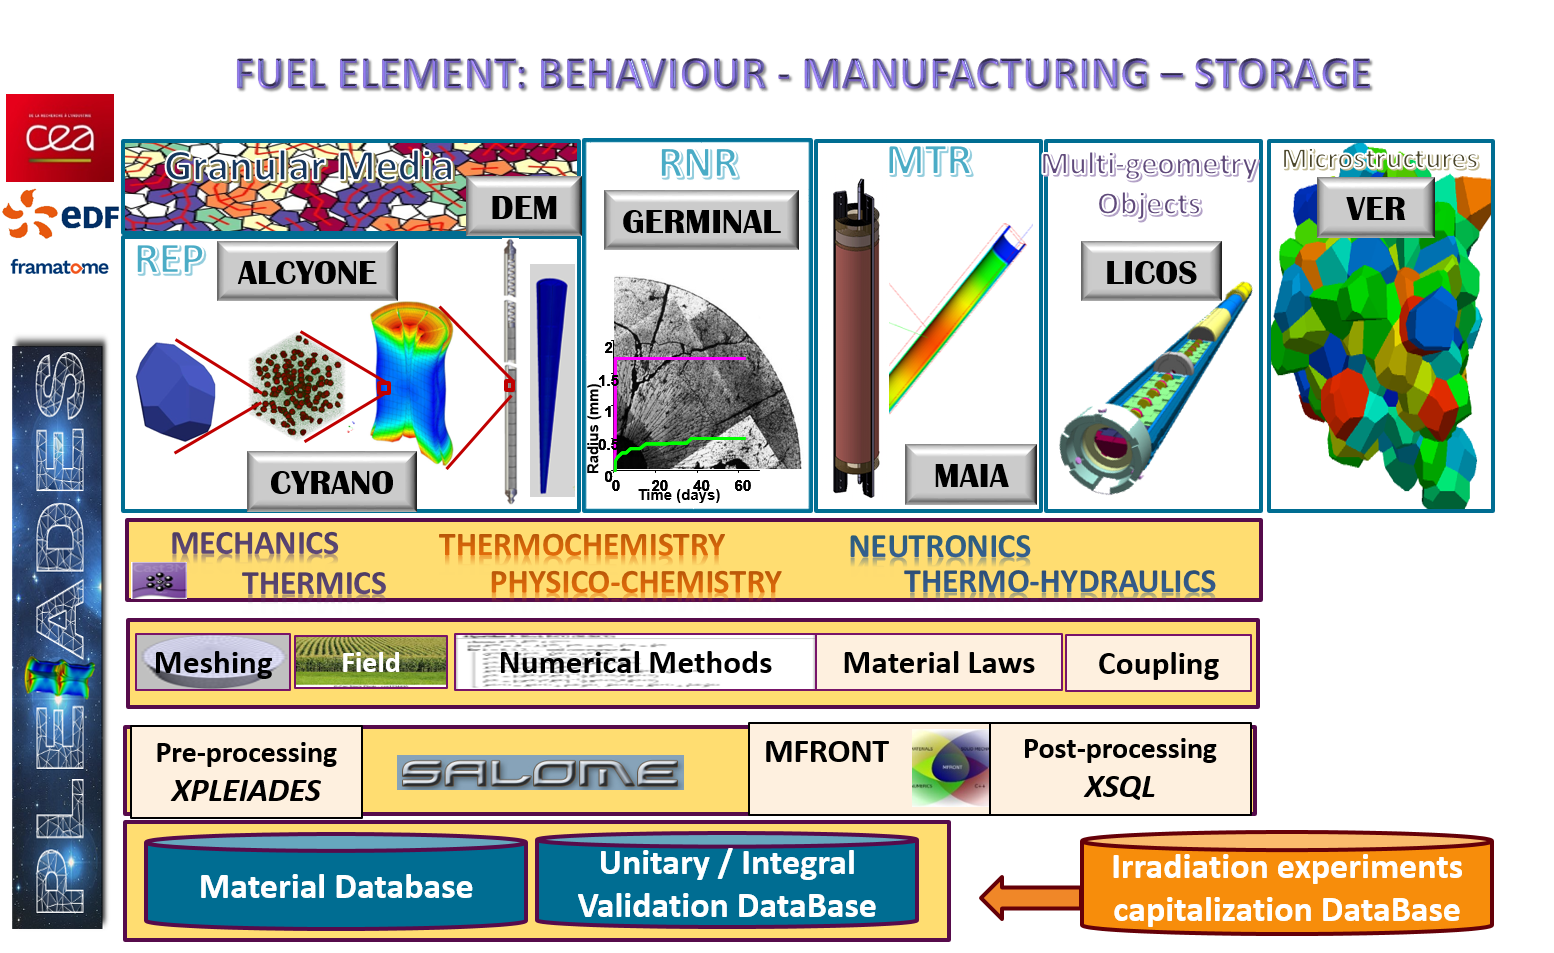
\includegraphics[trim = .2cm .2cm .2cm .6cm,clip,width=0.50\linewidth]{img/PLEIADES_2019_en.png}
  \end{center}
  \begin{itemize}
    \item A wide range of materials (ceramics, metals, composites).
    \item A wide range of mechanical phenomena and behaviours.
    \begin{itemize}
      \item Creep, swelling, irradiation effects, phase transitions, etc..
    \end{itemize}
    \item A wide range of mechanical loadings.
  \end{itemize}

\begin{textblock}{.40}(0.2,0.04)
\scalebox{.8}{\rotatebox{90}{
\begin{minipage}{7.cm}
\textcolor{blue}{The Pleiades Platform}
\end{minipage}}}
\end{textblock}

\begin{textblock}{.40}(0.8,0.08)
\scalebox{.8}{\rotatebox{90}{
\begin{minipage}{7.cm}
\textcolor{red}{Existing mechanical solver}\\\textcolor{red}{not well parallelized}
\end{minipage}}}
\end{textblock}
\end{frame}

\Titre{Goals of MFEM-MGIS}
\frame{
  \begin{itemize}
    \item Build a HPC general purpose non linear multi-physics
    library,\\
\hspace*{1cm}\textit{development began end of 2020.}
    \begin{itemize}
      \item Primary focus is \textbf{non linear solid mechanics} and
      \textbf{heat transfer}.
      \item Expected modelling (long-term): Shells, Beams,\\Phase-field
      approaches of brittle fracture, micromorphic models, Cosserat
      plasticity, strongly coupled thermo-chemical-mechanical or
      thermo-hydro-mechanical phenomena.
    \end{itemize}
\bigskip
    \item  A two-pillar library with \textit{opensource} commitment (\scalebox{0.8}{MFEM-MGIS \textit{LGPL 3.0}}):
    \begin{itemize}
      \item \texttt{MFEM:} HPC finite element solver. \scalebox{0.8}{\textit{(LGPL 2.1)}}
      \item \texttt{MGIS/MFront:} constitutive laws, material modelling. \scalebox{0.8}{\textit{(LGPL 3.0 / GPL 3.0)}}
    \end{itemize}
  \end{itemize}
}

\section{A small tutorial}
\Intercalaire{A small tutorial}


\begin{frame}[fragile]{What are we talking about ? \\
Example of end-user API}
  \begin{center}
%    \scalebox{0.7}{
      \begin{minipage}{\linewidth}
      \tiny
      \begin{Highlighting}[]
        \CommentTok{// loading the mesh and building the non linear problem}
        \NormalTok{mfem_mgis::NonLinearEvolutionProblem problem(}
        \NormalTok{    \{\{}\StringTok{"MeshFileName"}\NormalTok{, mesh_file\},  \{}\StringTok{"FiniteElementFamily"}\NormalTok{, }\StringTok{"H1"}\NormalTok{\},}
        \NormalTok{     \{}\StringTok{"FiniteElementOrder"}\NormalTok{, order\}, \{}\StringTok{"UnknownsSize"}\NormalTok{, dim\},}
        \NormalTok{     \{}\StringTok{"Hypothesis"}\NormalTok{, }\StringTok{"PlaneStrain"}\NormalTok{\}, \{}\StringTok{"Parallel"}\NormalTok{, parallel\}\});}
        \CommentTok{// associating names to element and boundary attributes (could be automated for some mesh formats)}
        \NormalTok{problem.setMaterialsNames(\{\{1, }\StringTok{"NotchedBeam"}\NormalTok{\}\});}
        \NormalTok{problem.setBoundariesNames(\{\{3, }\StringTok{"LowerBoundary"}\NormalTok{\}, \{4, }\StringTok{"SymmetryAxis"}\NormalTok{\}, \{2, }\StringTok{"UpperBoundary"}\NormalTok{\}\});}
        \CommentTok{// declaring behaviour integrators}
        \NormalTok{problem.}\NormalTok{addBehaviourIntegrator}\NormalTok{(}\StringTok{"Mechanics"}\NormalTok{, }\StringTok{"NotchedBeam"}\NormalTok{, library, behaviour);}
        \CommentTok{// setting the initial state of the materials}
        \KeywordTok{auto}\NormalTok{\& m1 = problem.getMaterial(}\StringTok{"NotchedBeam"}\NormalTok{);}
        \NormalTok{mgis::behaviour::setExternalStateVariable(m1.s0, }\StringTok{"Temperature"}\NormalTok{, }\FloatTok{293.15}\NormalTok{);}
        \NormalTok{...}
        \CommentTok{// defining boundary conditions, postprocessings and solver parameters}
        \NormalTok{problem.addUniformDirichletBoundaryCondition(\{\{}\StringTok{"Boundary"}\NormalTok{, }\StringTok{"LowerBoundary"}\NormalTok{\}, \{}\StringTok{"Component"}\NormalTok{, 1\}\}\});}
        \NormalTok{problem.addPostProcessing(}\StringTok{"ParaviewExportResults"}\NormalTok{, \{\{}\StringTok{"OutputFileName"}\NormalTok{, }\StringTok{"ssna303-displacements"}\NormalTok{\}\})};
        \KeywordTok{auto}\NormalTok{\& solver = problem.getSolver();}
        \NormalTok{...}
        \CommentTok{// loop over time step}
        \ControlFlowTok{for}\NormalTok{ (mfem\_mgis::}\DataTypeTok{size\_type}\NormalTok{ i = }\DecValTok{0}\NormalTok{; i != nsteps; ++i) \{}
        \CommentTok{  // updating the boundary values and resolution}
        \NormalTok{  ...}
        \NormalTok{  problem.solve(dt);}
        \NormalTok{  problem.update();}
        \NormalTok{  t += dt;}
        \NormalTok{\}}
      \end{Highlighting}
    \end{minipage}
    %    }
  \end{center}
  \begin{itemize}
    \item Instantiating \scalebox{0.8}{\texttt{NonLinearEvolutionProblem}} class is the
    main entry point.
    \item \textbf{Behaviour integrator} is the main new
    concept of {\tt MFEM/MGIS} .
  \end{itemize}
\end{frame}

\section{Design and features of the \texttt{MFEM-MGIS} project}
\Intercalaire{Design and features of the \texttt{MFEM-MGIS} project}

\Titre{MFront goals}
\begin{frame}
  \begin{center}
    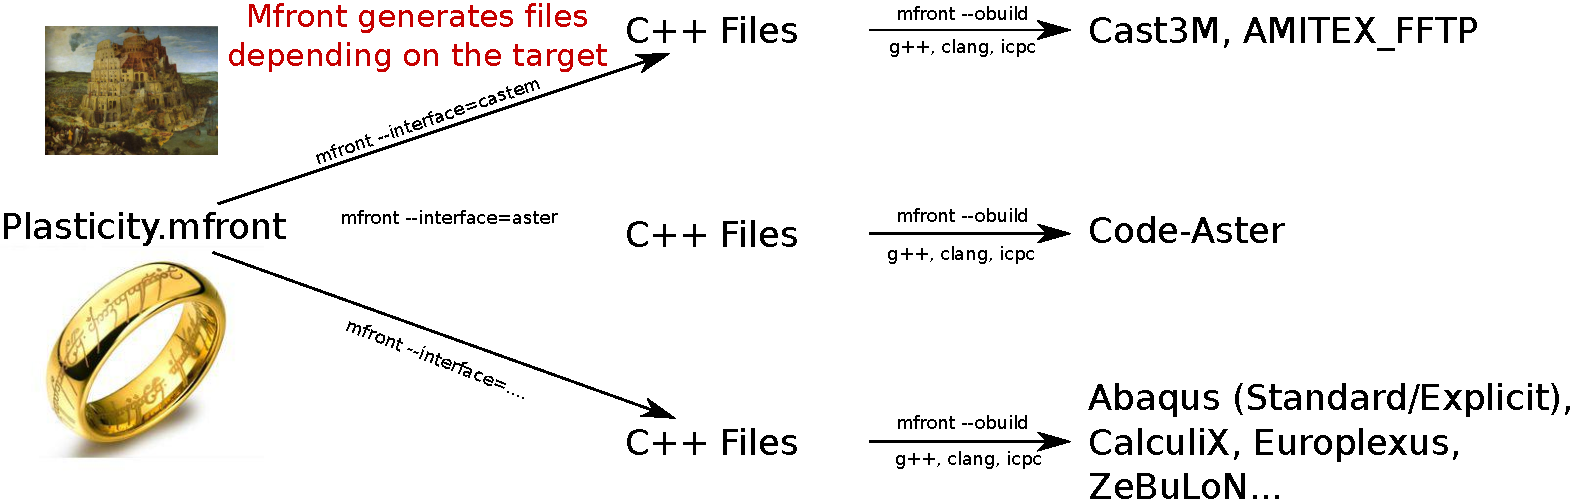
\includegraphics[width=0.55\textwidth]{img/MFrontPrinciple.pdf}
  \end{center}
  \begin{itemize}
    \item {\tt MFront} is a code generation tool dedicated to
    material knowledge (material properties, mechanical behaviours,
    point-wise models):
    \begin{itemize}
      \item Support for small and finite strain behaviours,
      cohesive zone models, {\bf generalised behaviours} (non local and
      or multiphysics).
    \end{itemize}
    \item Main goals:
    \begin{itemize}
      \item Numerical efficiency (see various benchmarks on
      the website).
      \item Portability and coupling capabilities ({\tt Cast3M}, {\tt Cyrano}, {\tt
        code\_aster}, {\tt Europlexus}, {\tt TMFTT}, {\tt AMITEX\_FFTP},
      {\tt Abaqus}, {\tt CalculiX}, {\tt MTest}).
      \item {\bf Ease of use}: {\em Longum iter est per
        praecepta, breve et efficax per exempla} (It's a long way by the
      rules, but short and efficient with examples).
    \end{itemize}
  \end{itemize}
\end{frame}

\Titre{The \texttt{MFrontGenericInterfaceSupport} project}
\begin{frame}
  \begin{center}
    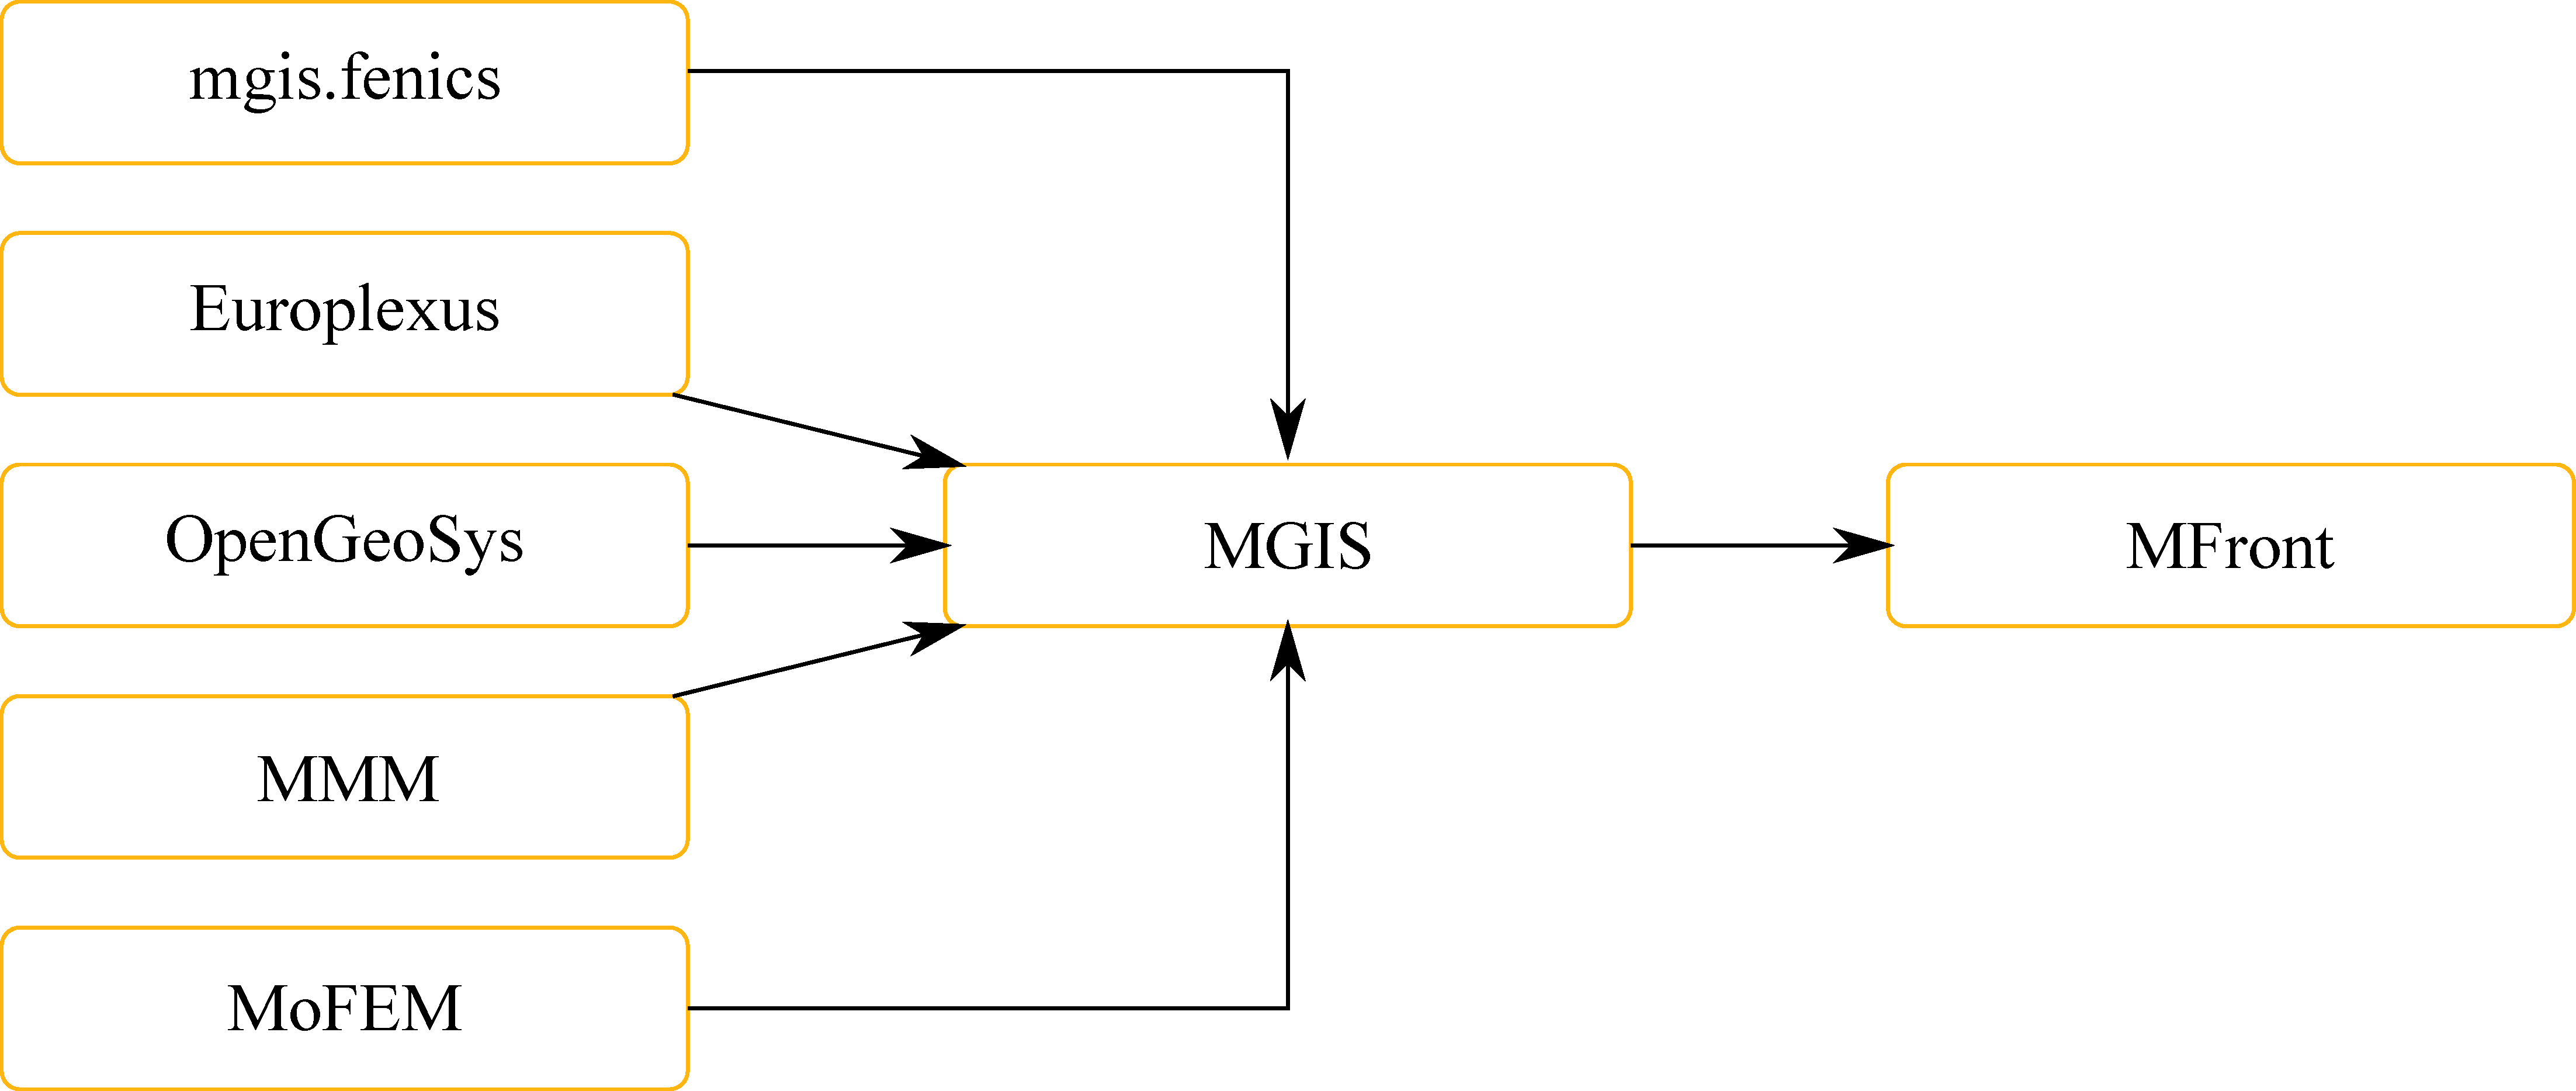
\includegraphics[width=0.75\textwidth]{img/mgis.pdf}
  \end{center}
  \begin{itemize}
    \item The {\tt MGIS} project provides classes on the solver
    side to retrieve {\bf metadata} from an {\tt MFront} behaviour and
    call the behaviour integration over a time step.
    \item Written in \texttt{C++}. Bindings exists for
    \texttt{C}, \texttt{Fortran2003}, \texttt{python}, \texttt{Julia}.
    \item Used/tested in \texttt{mgis.fenics},
    \texttt{OpenGeoSys}, \texttt{Manta}, \texttt{XPer}, \texttt{MoFEM},
    \texttt{Disk++}, \texttt{Kratos Multiphysics}, \texttt{JuliaFEM},
    \texttt{NairmMPM}, \texttt{esys.escript}, \texttt{DUNE},
    \texttt{OOFEM}, and more...
  \end{itemize}
\end{frame}

\begin{frame}[fragile]{The
    added value of \texttt{MFEM-MGIS}}
  \begin{itemize}
    \item Statement:
    \begin{itemize}
      \item \emph{Poor} support of multiple materials in
      \texttt{MFEM} for solid mechanics.
      \item \emph{No} support for functions on integration
      points for a given material (element attribute).
    \end{itemize}
    \item Proposed improvements:
    \begin{itemize}
      \item Add support for non linear behaviour integrators
      based on \texttt{MFront}.
      \item Add functions on integration points that depends on
      material identifier (element attribute).
      \item Simplified High-level API for end users (mechanics)
    \end{itemize}
    \item<2-> In practice:
    \begin{itemize}
      \item \texttt{MFEM-MGIS} is a library made up of
      \begin{enumerate}
        
        \item Classes that inherit from \texttt{MFEM}:\\ loops
        on elements, linear \& non-linear solvers, mesh management\ldots{}
        \item Classes that inherit from \texttt{MGIS}:
        materials management, internal variables, fill matrix
        entries\ldots{}
        \item Procedures for the end user to interact with MFEM
        \& MGIS
      \end{enumerate}
    \end{itemize}
    \item<3-> \texttt{MFEM-MGIS} is a C++17 opensource library:
    \begin{itemize}
      \item \url{https://github.com/thelfer/mfem-mgis}
      \item \url{https://github.com/latug0/mfem-mgis-examples}
    \end{itemize}
  \end{itemize}
\end{frame}

\begin{frame}{The
    role of behaviour integrators}
  \begin{center}
    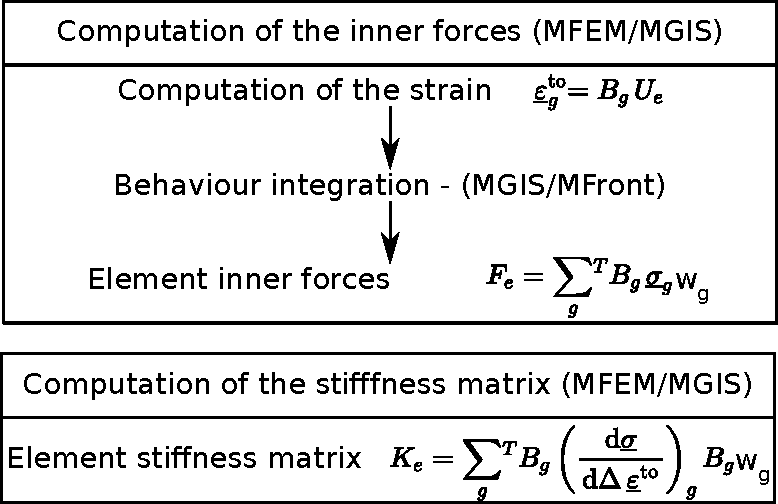
\includegraphics[width=0.6\textwidth]{img/behaviour-integrators.pdf}
  \end{center}
  \begin{itemize}
    \item Behaviour integrators are associated with a material
    identifier (element attribute).
    \item Behaviour integrators are called in the assembly loop
    over the elements for:
    \begin{itemize}
      \item the residual (contribution of the inner forces)
      \item the jacobian matrix (i.e.~the tangent stiffness
      matrix)
    \end{itemize}
  \end{itemize}
\end{frame}


%\begin{frame}[fragile]{Computation of the inner forces}
%  \protect\hypertarget{computation-of-the-inner-forces}{}
%  \begin{Shaded}
%    \begin{Highlighting}[]
%      \KeywordTok{template}\NormalTok{ \textless{}Hypothesis H\textgreater{}}
%      \DataTypeTok{void}\NormalTok{ SmallStrainMechanicalBehaviourIntegrator\textless{}H\textgreater{}::updateInnerForces(}
%      \NormalTok{      mfem::Vector \&Fe,}
%      \AttributeTok{const}\NormalTok{ mgis::span\textless{}}\AttributeTok{const}\NormalTok{ real\textgreater{} \&s,}
%      \AttributeTok{const}\NormalTok{ mfem::DenseMatrix \&dN,}
%      \AttributeTok{const}\NormalTok{ real w,}
%      \AttributeTok{const} \DataTypeTok{size\_type}\NormalTok{ ni) }\AttributeTok{const}\NormalTok{ \{}
%      \KeywordTok{constexpr} \AttributeTok{const} \KeywordTok{auto}\NormalTok{ icste = }\FloatTok{0.70710678118654752440}\NormalTok{;}
%      \KeywordTok{static\_assert}\NormalTok{(H == Hypothesis::TRIDIMENSIONAL, }\StringTok{"unsupported hypothesis"}\NormalTok{);}
%      \ControlFlowTok{if} \KeywordTok{constexpr}\NormalTok{ (H == Hypothesis::TRIDIMENSIONAL) \{}
%      \AttributeTok{const} \KeywordTok{auto}\NormalTok{ nnodes = dN.NumRows();}
%      \AttributeTok{const} \KeywordTok{auto}\NormalTok{ nx = ni;}
%      \AttributeTok{const} \KeywordTok{auto}\NormalTok{ ny = ni + nnodes;}
%      \AttributeTok{const} \KeywordTok{auto}\NormalTok{ nz = ni + }\DecValTok{2}\NormalTok{ * nnodes;}
%      \NormalTok{      real B[}\DecValTok{6}\NormalTok{][}\DecValTok{3}\NormalTok{] = \{\{dN(ni, }\DecValTok{0}\NormalTok{), }\DecValTok{0}\NormalTok{, }\DecValTok{0}\NormalTok{\},                          }\CommentTok{//}
%      \NormalTok{                      \{}\DecValTok{0}\NormalTok{, dN(ni, }\DecValTok{1}\NormalTok{), }\DecValTok{0}\NormalTok{\},                          }\CommentTok{//}
%      \NormalTok{                      \{}\DecValTok{0}\NormalTok{, }\DecValTok{0}\NormalTok{, dN(ni, }\DecValTok{2}\NormalTok{)\},                          }\CommentTok{//}
%      \NormalTok{                      \{dN(ni, }\DecValTok{1}\NormalTok{) * icste, dN(ni, }\DecValTok{0}\NormalTok{) * icste, }\DecValTok{0}\NormalTok{\},  }\CommentTok{// xy}
%      \NormalTok{                      \{dN(ni, }\DecValTok{2}\NormalTok{) * icste, }\DecValTok{0}\NormalTok{, dN(ni, }\DecValTok{0}\NormalTok{) * icste\},  }\CommentTok{// xz}
%      \NormalTok{                      \{}\DecValTok{0}\NormalTok{, dN(ni, }\DecValTok{2}\NormalTok{) * icste, dN(ni, }\DecValTok{1}\NormalTok{) * icste\}\}; }\CommentTok{// yz}
%      \NormalTok{      Fe[nx] += w * (B[}\DecValTok{0}\NormalTok{][}\DecValTok{0}\NormalTok{] * s[}\DecValTok{0}\NormalTok{] + B[}\DecValTok{1}\NormalTok{][}\DecValTok{0}\NormalTok{] * s[}\DecValTok{1}\NormalTok{] + B[}\DecValTok{2}\NormalTok{][}\DecValTok{0}\NormalTok{] * s[}\DecValTok{2}\NormalTok{] +}
%      \NormalTok{                     B[}\DecValTok{3}\NormalTok{][}\DecValTok{0}\NormalTok{] * s[}\DecValTok{3}\NormalTok{] + B[}\DecValTok{4}\NormalTok{][}\DecValTok{0}\NormalTok{] * s[}\DecValTok{4}\NormalTok{] + B[}\DecValTok{5}\NormalTok{][}\DecValTok{0}\NormalTok{] * s[}\DecValTok{5}\NormalTok{]);}
%      \NormalTok{      Fe[ny] += w * (B[}\DecValTok{0}\NormalTok{][}\DecValTok{1}\NormalTok{] * s[}\DecValTok{0}\NormalTok{] + B[}\DecValTok{1}\NormalTok{][}\DecValTok{1}\NormalTok{] * s[}\DecValTok{1}\NormalTok{] + B[}\DecValTok{2}\NormalTok{][}\DecValTok{1}\NormalTok{] * s[}\DecValTok{2}\NormalTok{] +}
%      \NormalTok{                     B[}\DecValTok{3}\NormalTok{][}\DecValTok{1}\NormalTok{] * s[}\DecValTok{3}\NormalTok{] + B[}\DecValTok{4}\NormalTok{][}\DecValTok{1}\NormalTok{] * s[}\DecValTok{4}\NormalTok{] + B[}\DecValTok{5}\NormalTok{][}\DecValTok{1}\NormalTok{] * s[}\DecValTok{5}\NormalTok{]);}
%      \NormalTok{      Fe[nz] += w * (B[}\DecValTok{0}\NormalTok{][}\DecValTok{2}\NormalTok{] * s[}\DecValTok{0}\NormalTok{] + B[}\DecValTok{1}\NormalTok{][}\DecValTok{2}\NormalTok{] * s[}\DecValTok{1}\NormalTok{] + B[}\DecValTok{2}\NormalTok{][}\DecValTok{2}\NormalTok{] * s[}\DecValTok{2}\NormalTok{] +}
%      \NormalTok{                     B[}\DecValTok{3}\NormalTok{][}\DecValTok{2}\NormalTok{] * s[}\DecValTok{3}\NormalTok{] + B[}\DecValTok{4}\NormalTok{][}\DecValTok{2}\NormalTok{] * s[}\DecValTok{4}\NormalTok{] + B[}\DecValTok{5}\NormalTok{][}\DecValTok{2}\NormalTok{] * s[}\DecValTok{5}\NormalTok{]);}
%      \NormalTok{    \}}
%      \NormalTok{  \}  }\CommentTok{// end of updateInnerForces}
%    \end{Highlighting}
%  \end{Shaded}
%  
%  \begin{itemize}
%    
%    \item
%    Note: code from the first versions of \texttt{mfem-mgis}
%    \item
%    The \texttt{B} matrix have numerous null entries.
%    
%    \begin{itemize}
%      
%      \item
%      The computation of \texttt{F} can easily be optimised.
%    \end{itemize}
%  \end{itemize}
%\end{frame}
%
%\begin{frame}[fragile]{Computation of the inner forces (optimized)}
%  \protect\hypertarget{computation-of-the-inner-forces-optimized}{}
%  \begin{Shaded}
%    \begin{Highlighting}[]
%      \KeywordTok{template}\NormalTok{ \textless{}Hypothesis H\textgreater{}}
%      \DataTypeTok{void}\NormalTok{ SmallStrainMechanicalBehaviourIntegrator\textless{}H\textgreater{}::updateInnerForces(}
%      \NormalTok{      mfem::Vector \&Fe,}
%      \AttributeTok{const}\NormalTok{ mgis::span\textless{}}\AttributeTok{const}\NormalTok{ real\textgreater{} \&s,}
%      \AttributeTok{const}\NormalTok{ mfem::DenseMatrix \&dN,}
%      \AttributeTok{const}\NormalTok{ real w,}
%      \AttributeTok{const} \DataTypeTok{size\_type}\NormalTok{ ni) }\AttributeTok{const}\NormalTok{ \{}
%      \KeywordTok{constexpr} \AttributeTok{const} \KeywordTok{auto}\NormalTok{ icste = }\FloatTok{0.70710678118654752440}\NormalTok{;}
%      \KeywordTok{static\_assert}\NormalTok{(H == Hypothesis::TRIDIMENSIONAL, }\StringTok{"unsupported hypothesis"}\NormalTok{);}
%      \ControlFlowTok{if} \KeywordTok{constexpr}\NormalTok{ (H == Hypothesis::TRIDIMENSIONAL) \{}
%      \AttributeTok{const} \KeywordTok{auto}\NormalTok{ nnodes = dN.NumRows();}
%      \AttributeTok{const} \KeywordTok{auto}\NormalTok{ nx = ni;}
%      \AttributeTok{const} \KeywordTok{auto}\NormalTok{ ny = ni + nnodes;}
%      \AttributeTok{const} \KeywordTok{auto}\NormalTok{ nz = ni + }\DecValTok{2}\NormalTok{ * nnodes;}
%      \NormalTok{      real B[}\DecValTok{6}\NormalTok{][}\DecValTok{3}\NormalTok{] = \{\{dN(ni, }\DecValTok{0}\NormalTok{), }\DecValTok{0}\NormalTok{, }\DecValTok{0}\NormalTok{\},                          }\CommentTok{//}
%      \NormalTok{                      \{}\DecValTok{0}\NormalTok{, dN(ni, }\DecValTok{1}\NormalTok{), }\DecValTok{0}\NormalTok{\},                          }\CommentTok{//}
%      \NormalTok{                      \{}\DecValTok{0}\NormalTok{, }\DecValTok{0}\NormalTok{, dN(ni, }\DecValTok{2}\NormalTok{)\},                          }\CommentTok{//}
%      \NormalTok{                      \{dN(ni, }\DecValTok{1}\NormalTok{) * icste, dN(ni, }\DecValTok{0}\NormalTok{) * icste, }\DecValTok{0}\NormalTok{\},  }\CommentTok{// xy}
%      \NormalTok{                      \{dN(ni, }\DecValTok{2}\NormalTok{) * icste, }\DecValTok{0}\NormalTok{, dN(ni, }\DecValTok{0}\NormalTok{) * icste\},  }\CommentTok{// xz}
%      \NormalTok{                      \{}\DecValTok{0}\NormalTok{, dN(ni, }\DecValTok{2}\NormalTok{) * icste, dN(ni, }\DecValTok{1}\NormalTok{) * icste\}\}; }\CommentTok{// yz}
%      \NormalTok{      Fe[nx] += w * (B[}\DecValTok{0}\NormalTok{][}\DecValTok{0}\NormalTok{] * s[}\DecValTok{0}\NormalTok{] + B[}\DecValTok{3}\NormalTok{][}\DecValTok{0}\NormalTok{] * s[}\DecValTok{3}\NormalTok{] + B[}\DecValTok{4}\NormalTok{][}\DecValTok{0}\NormalTok{] * s[}\DecValTok{4}\NormalTok{]);}
%      \NormalTok{      Fe[ny] += w * (B[}\DecValTok{1}\NormalTok{][}\DecValTok{1}\NormalTok{] * s[}\DecValTok{1}\NormalTok{] + B[}\DecValTok{3}\NormalTok{][}\DecValTok{1}\NormalTok{] * s[}\DecValTok{3}\NormalTok{] + B[}\DecValTok{5}\NormalTok{][}\DecValTok{1}\NormalTok{] * s[}\DecValTok{5}\NormalTok{]);}
%      \NormalTok{      Fe[nz] += w * (B[}\DecValTok{2}\NormalTok{][}\DecValTok{2}\NormalTok{] * s[}\DecValTok{2}\NormalTok{] + B[}\DecValTok{4}\NormalTok{][}\DecValTok{2}\NormalTok{] * s[}\DecValTok{4}\NormalTok{] + B[}\DecValTok{5}\NormalTok{][}\DecValTok{2}\NormalTok{] * s[}\DecValTok{5}\NormalTok{]);}
%      \NormalTok{    \}}
%      \NormalTok{  \}  }\CommentTok{// end of updateInnerForces}
%    \end{Highlighting}
%  \end{Shaded}
%  
%  \begin{itemize}
%    
%    \item
%    Note: code from the first versions of \texttt{mfem-mgis}
%  \end{itemize}
%\end{frame}

\begin{frame}{Behaviour
    integrators}
  \begin{itemize}
    \item Behaviour integrators are meant to:
    \begin{itemize}
      \item Compute the gradients from unknowns (using the
      \(B\) matrix).
      \item Handle the state variables.
      \item Call the behaviour integration.
      \item Compute the inner forces from the thermodynamic
      forces.
      \item Compute the stiffness matrix from the consistent
      tangent operator blocks.
    \end{itemize}
  \end{itemize}
  \begin{itemize}
    \item All those steps depends on:
    \begin{itemize}
      \item Kind of problem described (mechanics, heat
      transfer).
      \item Symmetry of the material (isotropic or
      orthotropic).
      \item Modelling hypotheses: \(3D\), plane strain,
      plane stress, axisymmetry \ldots
    \end{itemize}
  \end{itemize}
  \begin{itemize}
    \item The writting of behaviour integrators is tedious and
    error-prone and shall be done with care.
    \begin{itemize}
      \item However, specific behaviour integrators gives
      access to pieces of physics.
      \item Code generation to the rescue !
    \end{itemize}
  \end{itemize}
\end{frame}

\begin{frame}[fragile]{The
    \texttt{behaviour-integrator} code
    generator}
  \begin{itemize}
    \item Aim of this code-generator
    \begin{itemize}
      \item Generate behaviour integrators from definition of the gradients.
      \item Automated code factorisation/optimisation (no sparse matrix multiply).
      \item Avoid coding errors due to tedious formula.
    \end{itemize}
    \item Machinery
    \begin{itemize}
      \item Based on the \texttt{GiNaC} for symbolic
      computations in \texttt{C++}
      \item Current scope: isotropic and orthotropic, small
      and finite strain behaviours in plane strain, plane stress and
      tridimensional hypotheses.
    \end{itemize}
    \item Extensions (to come)
    \begin{itemize}
      \item Support of axisymmetry
      \item Non linear heat transfer, non linear diffusion.
      \item Can be extended to other non-linear models, wide
      range of phenomena.
    \end{itemize}
  \end{itemize}
\end{frame}

\section{Feed-backs on some issues using {\tt MFEM}}
\Intercalaire{Feed-backs on some issues using {\tt MFEM}}

\Titre{Issues related to\\\hspace*{1cm}the behaviour integration step}
\frame{
  \begin{itemize}
    \item The integration of the mechanical behaviour is a {\bf
      complex} kernel solving a system of ordinary differential
    equations which can {\bf fail}.
    \item Problem: the {\tt
      NonlinearFormIntegrator::AssembleElementVector} and {\tt
      NonlinearFormIntegrator::AssembleElementGrad} does not handle
    failures.
    \item<2-> As a work-around, we derived our own Newton
    algorithm which separates the behaviour integration step from
    residual and stiffness assemblies.
    \begin{itemize}
      \item This solution seems compatible with
      partial assembly (untested).
      \item This work-around  {\bf does not work with {\tt
        PETSc}}.
    \end{itemize}
    \item<2-> More generally, we started a discussion on
    how to improve the robustness of operators in {\tt MFEM}:
    \begin{itemize}
      \item \url{https://github.com/mfem/mfem/issues/2139}
    \end{itemize}
  \end{itemize}
}

\Titre{Dirichlet boundary conditions} \frame{
  \begin{center}
    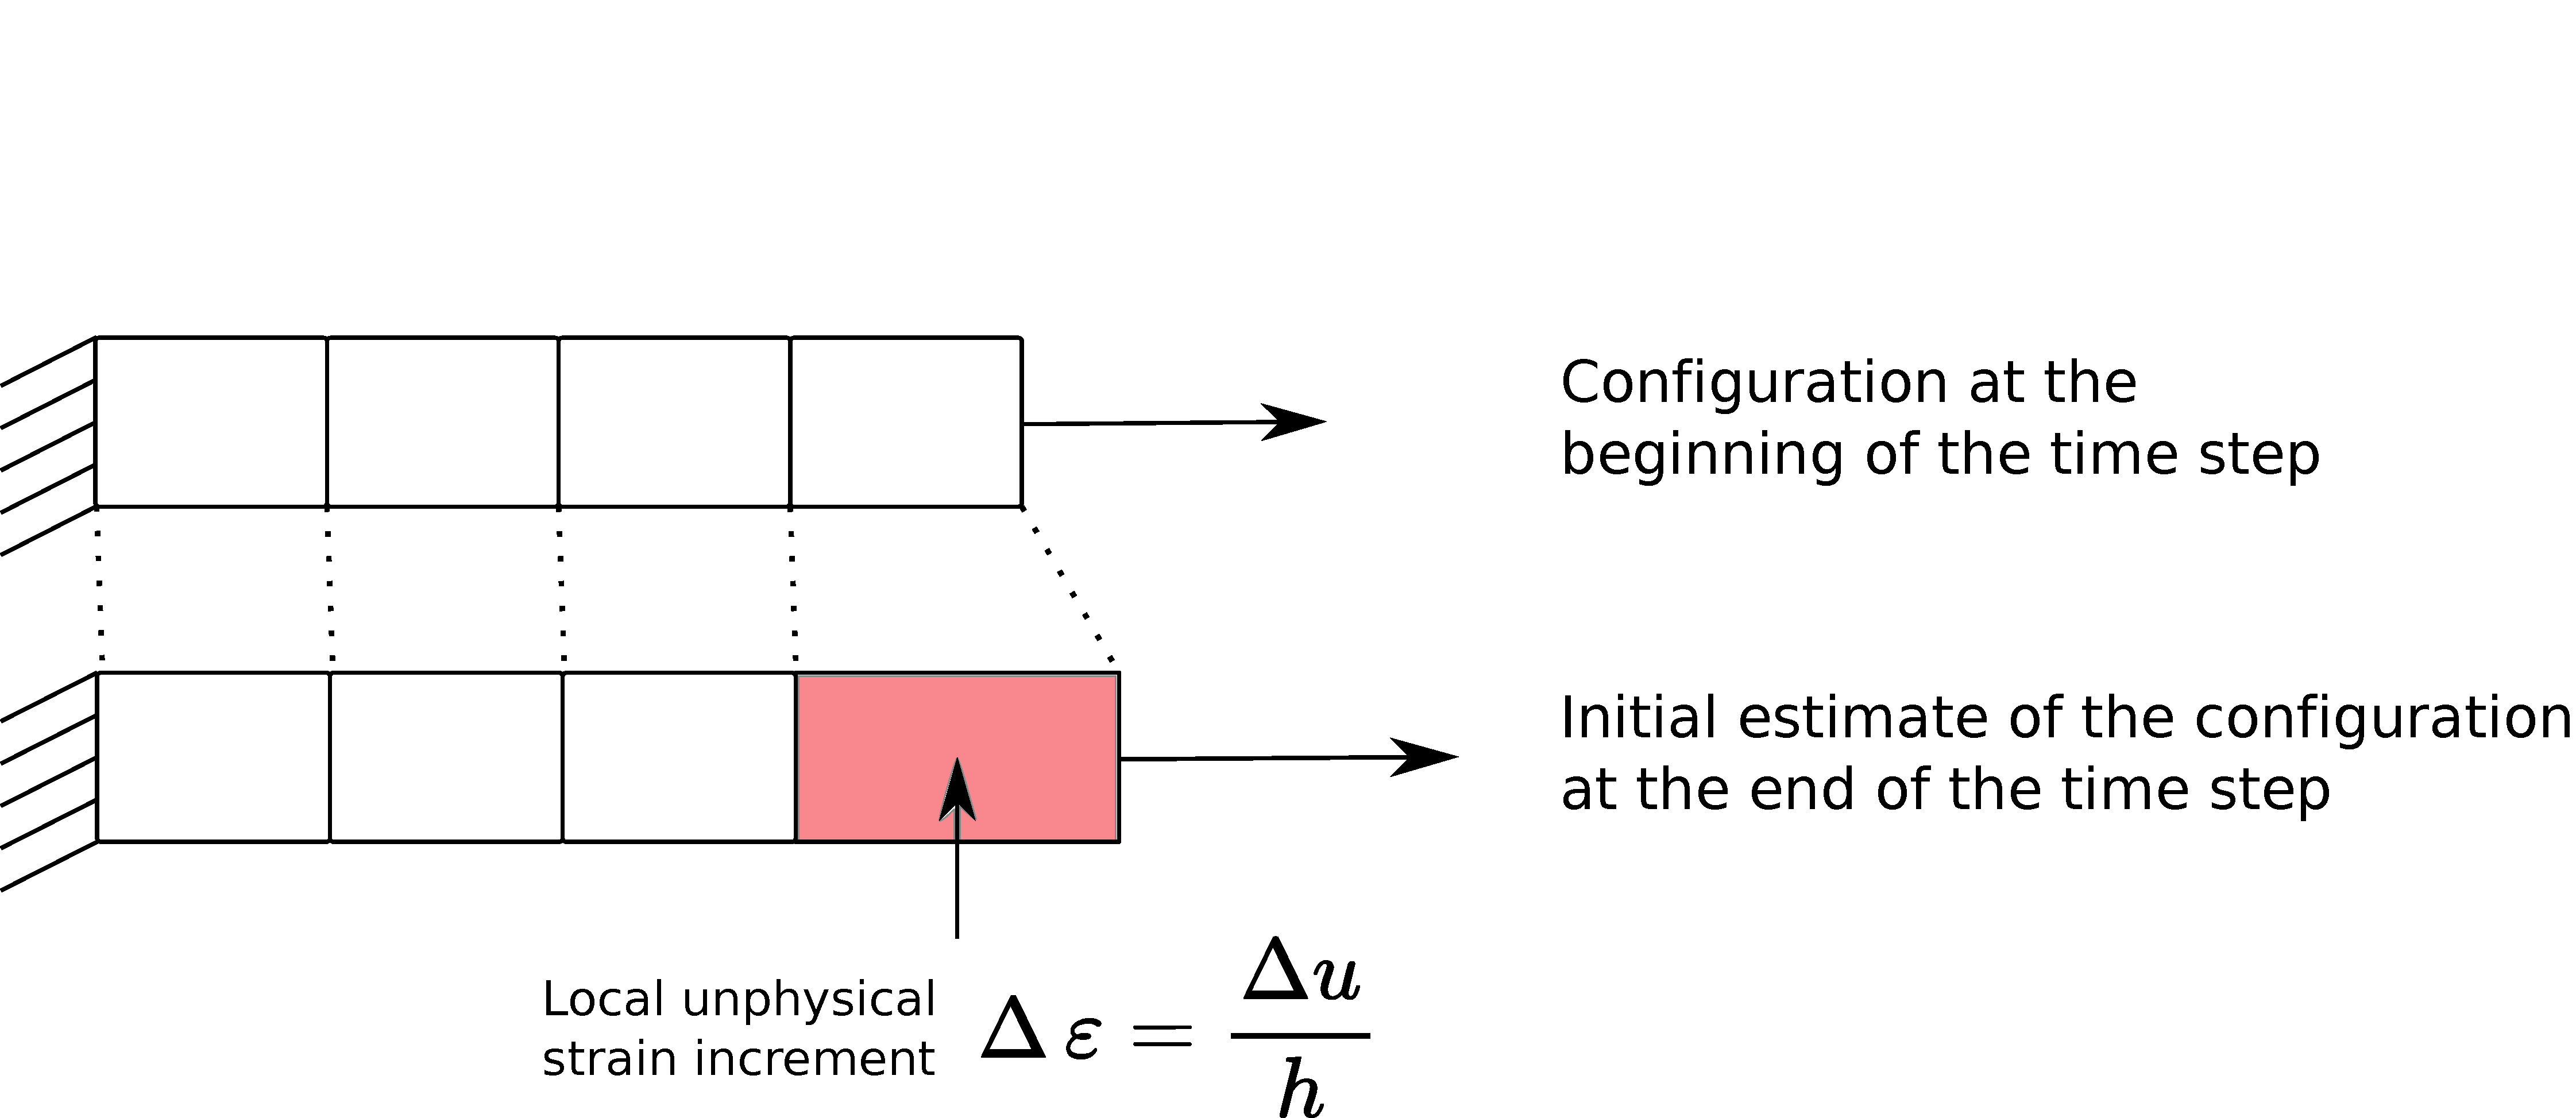
\includegraphics[width=0.65\textwidth]{img/DirichletBoundaryConditionIssue.pdf}
  \end{center}
  \begin{itemize}
    \item Imposing the boundary Dirichlet in {\tt MFEM} leads
    to unphysically strain increments on elements near the boundary at
    the first iteration:
    \begin{itemize}
      \item The problem becomes more and more import as the
      mesh is refined.
      \item In finite strain, this leads to severe divergence
      of the Newton algorithm du to the geometric stiffness matrix.
    \end{itemize}
    \item<2-> In most \textbf{mechanical} solvers, a \textbf{prediction} of the
    solution based on the tangent problem is performed.
    \begin{itemize}
      \item We were not able to implement this prediction so far.
      \item \url{https://github.com/mfem/mfem/issues/2174}
    \end{itemize}
  \end{itemize}
}

\section{Examples}
\Intercalaire{Examples}

\begin{frame}{Non linear case \\\hspace*{1cm} Finite strain}
\begin{textblock}{.9}(0.02,0.1)
  \begin{block}{Case description}
    \begin{itemize}
      \item Uniaxial tensile test on a notched beam
      \item Imposed displacement: right of the beam
      \item Symmetry conditions at: left position, down position 
      \item Non-linear elastoplastic modelling, finite strain
    \end{itemize}
  \end{block}
\end{textblock}
\begin{textblock}{.5}(0.,0.5)
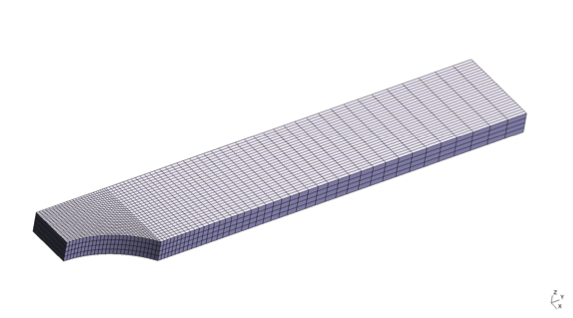
\includegraphics[width=0.8\textwidth]{img/ssna303-geom.png}\\
\hspace*{3mm}{\small 3D geometry of the notched beam}
\end{textblock}
\begin{textblock}{.5}(0.44,0.49)
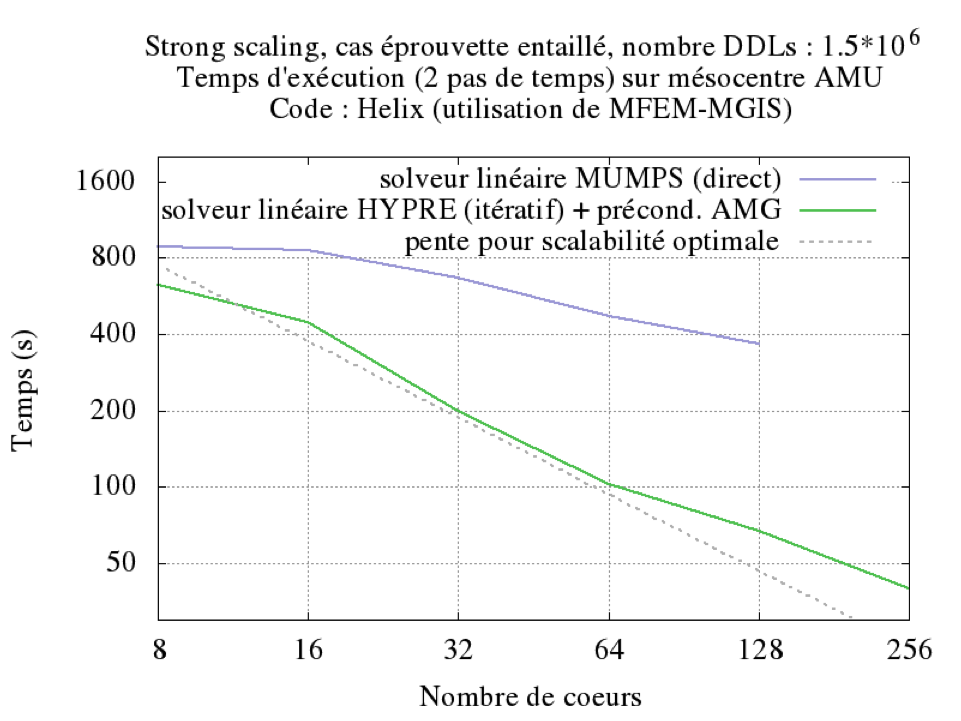
\includegraphics[width=0.9\textwidth]{img/ssna303_scaling.png}
\end{textblock}
\end{frame}


\begin{frame}{Periodic
    Representative Volume Element (RVE)\\\hspace*{1cm}
    Pratical setting}
  \begin{block}{Test
      case setting - elastic model}
    \protect\hypertarget{test-case-setting---elastic-model}{}
    \begin{itemize}
      \item Two isotropic materials, each one filling half of
      a cube
      \item Aim : compare against \textbf{\texttt{MFEM-MGIS}}
      results against \textbf{analytical} results
      \begin{itemize}
        \item considering 3 cases with uniaxial strain
        \item considering 3 cases with shear test
      \end{itemize}
    \end{itemize}
  \end{block}
  \begin{block}{Mesh
      and result} \vspace*{-5mm}
    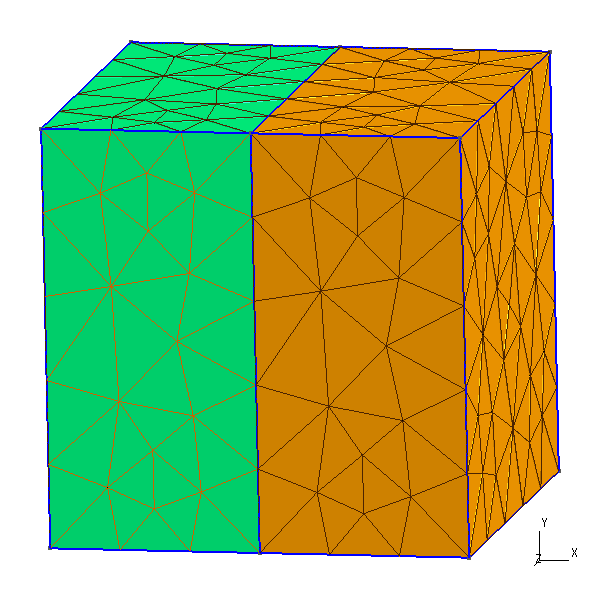
\includegraphics[width=0.33\textwidth]{img/cube_2mat.png}
    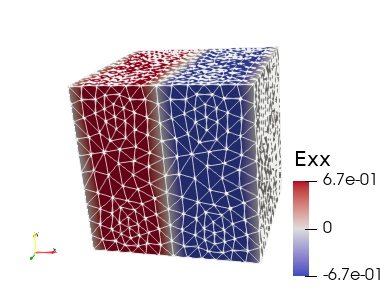
\includegraphics[width=0.49\textwidth]{img/cube_2mat_exx.png}
    \vspace*{-1mm}
  \end{block}
\end{frame}

\begin{frame}{Periodic
    RVE - Numerical results on 32 cores}
  \begin{block}{Properties}
    \begin{itemize}
      \item 14 million unknowns, elastic modelling
      \item Ref. case on \emph{32 cores} - skylake @
      mesocentre Aix-Marseille University
      \item Main linear solver: Conj. Gradient (iterative),
      no preconditioner used
    \end{itemize}
  \end{block}
  \vspace*{2mm}
  \begin{block}{Timings}
    \begin{itemize}
      \item MFEM linear solve
      \begin{itemize}
        \item total \textbf{166s}, ~~ matrix assembly 39s,
        ~~ CGsolver 120s
      \end{itemize}
      \item MFEM non-linear solve - residual form, a single
      newton iteration
      \begin{itemize}
        \item total \textbf{179s}, ~~ matrix assembly 53s,
        ~~ CGsolver 117s
      \end{itemize}
      \item MFEM-MGIS non-linear solve - residual form, a
      single newton iteration
      \begin{itemize}
        \item total \textbf{188s}, ~~ matrix assembly 42s,
        ~~ CGsolver 133s
      \end{itemize}
      \item Overheads due to MFEM-MGIS are low
      \begin{itemize}
        \item Due to: read/write to memory buffers,
        function calls for assembly
      \end{itemize}
    \end{itemize}
  \end{block}
\end{frame}

\begin{frame}{Periodic
    REV - Strong Scaling}
  \begin{block}{Strong
      scaling}
    \begin{itemize}
      \item Using MFEM-MGIS non-linear solve
      \item Strong scaling from 32 to 256 cores
      \item Scalable parallelism observed
    \end{itemize}
  \end{block}
  \begin{block}{}
    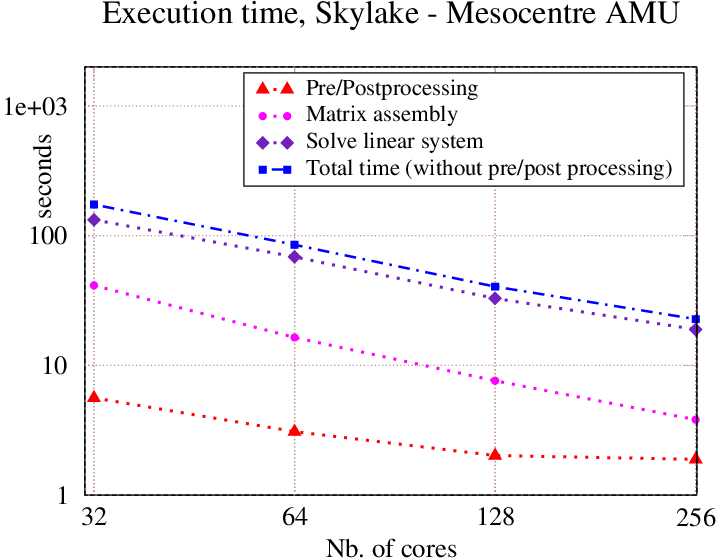
\includegraphics[width=0.4\textwidth]{img/bench_3.png}
    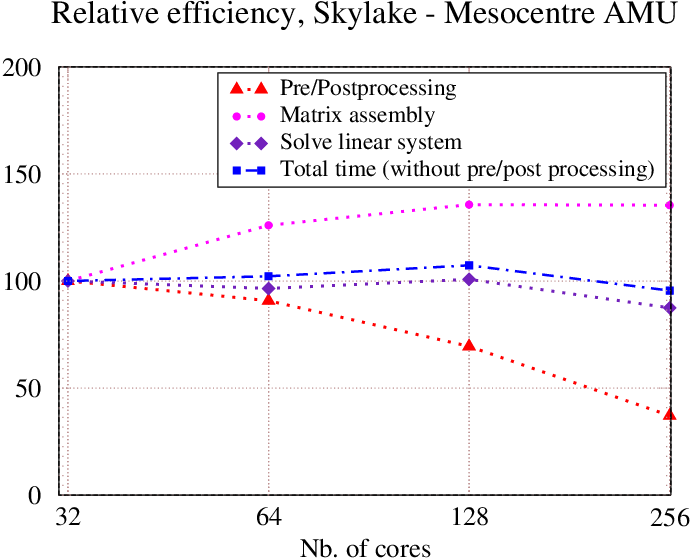
\includegraphics[width=0.4\textwidth]{img/bench_4.png}
  \end{block}
\end{frame}

\begin{frame}{Periodic
    REV - Modelling inclusions}
  \begin{block}{MFEM contributions \& coupling}
    \begin{itemize}
      \item using as input : 3D periodic \texttt{gmsh} meshes (public MFEM contrib)
      \item read/write MED files (private development)
      \item in progress : using \texttt{netgen} to get REV meshes (\texttt{gmsh} format)
    \end{itemize}
  \end{block}
  \begin{block}{Large runs}
    \hspace*{2cm}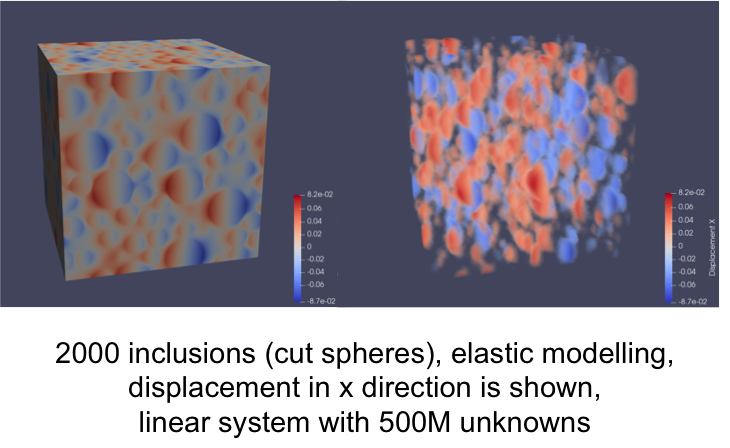
\includegraphics[width=0.6\textwidth]{img/REV_2000inc.png}
  \end{block}
\begin{textblock}{.2}(0.78,0.68)
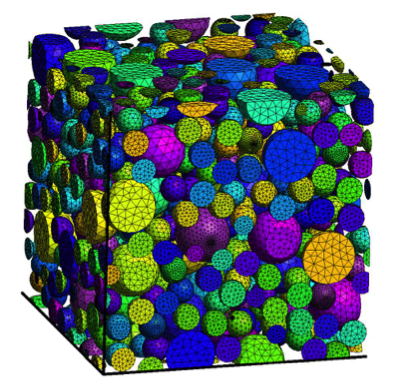
\includegraphics[width=\textwidth]{img/polydisperse.png}
\end{textblock}
\end{frame}


\section{Conclusions and perspectives}
\Intercalaire{Conclusions and perspectives}

\Titre{Conclusions and perspectives} \frame{
  \begin{itemize}
    \item What was done ?
    \begin{itemize}
      \item High level declarative API suitable for
      engineering studies and upcoming integration in the {\tt PLEIADES}
      platform.
      \begin{itemize}
        \item {\tt MFEM}' API still accessible user a lower
        level API (not shown here)
      \end{itemize}
      \item Multi-material support
      \item Ability to handle arbitrary complex small and
      finite strain behaviours:
      \begin{itemize}
        \item All behaviours are set at runtime
        (dynamically loaded libraries).
      \end{itemize}
    \end{itemize}
    \item<2-> What comes next ?
    \begin{itemize}
      \item Overall robustness of the code (critical).
      \item Prediction and handling of the Dirichlet boundary
      conditions (critical).
      \item Provide more examples (urgent).
      \item Extension to other physical phenomea (non linear
      heat-transfer, diffusion, non local mechanics). \textit{Should be
        easy} using code generation of behaviour integrators .
      \item Adaptative mesh refinements (requires new data
      structures in MGIS).
      \item Additional boundary conditions, including contact
      with friction.
      \item Port to GPUs (requires tremendous work on the
      MFront and MGIS side).
      \item Support for partial assembly (if possible ...),
      chekpoint/restart.
    \end{itemize}
  \end{itemize}
}


\DernierePage{ \vspace*{1.5cm} \hspace*{-1.2cm}
  \scalebox{0.9}{
    \begin{minipage}[h]{0.75\textwidth}
      \begin{center}
        \textcolor{white}{ Thank you for your
          attention.\\ Time for discussion !\\
          \small{\url{https://github.com/thelfer/mfem-mgis}}\\
          \small{\url{https://github.com/thelfer/MFrontGenericInterfaceSupport}}\\
          \small{\url{https://github.com/thelfer/mfem-mgis}}\\
          \small{\url{https://tfel.sourceforge.net}}\\
          \small{\url{https://www.researchgate.net/project/TFEL-MFront}}\\
          \small{\url{https://twitter.com/TFEL_MFront}}\\
          \small{\href{mailto:tfel-contact@cea.fr}{tfel-contact@cea.fr}}
        }
      \end{center}
    \end{minipage}
  }
  \hspace*{-5cm}
%  \vspace{-1.5cm}
  \scalebox{1}{
    \begin{minipage}[h]{0.95\textwidth}
      \textcolor{white}{The development
        of \texttt{MFront} is supported \\
        financially by CEA, EDF and Framatome \\
        in the framework of the \texttt{PLEIADES} project.
      }
    \end{minipage}
  }
}

\backupbegin
\begin{frame}{Non linear resolution\\\hspace*{1cm} in solid mechanics}
  \begin{itemize}
     \item    Mechanical equilibrium:
    find\(\Delta\ensuremath{\mathbb{\uppercase{\vec{u}}}}\) such as: \[
    \ensuremath{\ensuremath{\mathbb{\uppercase{\vec{R}}}}}{\left(\Delta\ensuremath{\mathbb{\uppercase{\vec{u}}}}\right)}=\ensuremath{\mathbb{\uppercase{\vec{O}}}}\quad\text{
      avec
    }\quad\ensuremath{\ensuremath{\mathbb{\uppercase{\vec{R}}}}}{\left(\Delta\ensuremath{\mathbb{\uppercase{\vec{u}}}}\right)}=\ensuremath{\ensuremath{\mathbb{\uppercase{\vec{F}}}}_{i}}{\left(\Delta\ensuremath{\mathbb{\uppercase{\vec{u}}}}\right)}-\ensuremath{\ensuremath{\mathbb{\uppercase{\vec{F}}}}_{e}}
    \] 
    \item Resolution using the Newton-Raphson algorithm: \[ 
    \Delta\ensuremath{\mathbb{\uppercase{\vec{u}}}}^{n+1}=\Delta\ensuremath{\mathbb{\uppercase{\vec{u}}}}^{n}-\ensuremath{\underline{\underline{\mathbf{\mathbb{K}}}}}^{-1}.\ensuremath{\ensuremath{\mathbb{\uppercase{\vec{R}}}}}{\left(\Delta\ensuremath{\mathbb{\uppercase{\vec{u}}}}^{n}\right)}
    \] 
        \item  Element contribution to inner forces: \[
    \ensuremath{\ensuremath{\mathbb{\uppercase{\vec{F}}}}_{i}^{e}}= \sum_{i=1}^{N^{G}} {\left(\ensuremath{\ensuremath{\underline{\mathbf{\sigma}}}}_{t+\Delta\,t}{\left(\Delta\ensuremath{\ensuremath{\underline{\mathbf{\epsilon}}}^{\mathit{to}}}{\left(\vec{\eta}_{i}\right)},\Delta\, t\right)}\colon\ensuremath{\underline{\underline{\mathbf{B}}}}{\left(\vec{\eta}_{i}\right)}\right)}w_{i}
    \]
        \item    Element contribution to the stiffness: \[
    \ensuremath{\underline{\underline{\mathbf{\mathbb{K}}}}}^{e}=\displaystyle\sum_{i=1}^{N^{G}}
    \mbox{}^{t}\ensuremath{\underline{\underline{\mathbf{B}}}}{\left(\vec{\eta}_{i}\right)}\colon\frac{\displaystyle\partial\,\Delta\ensuremath{\ensuremath{\underline{\mathbf{\sigma}}}}}{\displaystyle\partial\,\Delta\ensuremath{\ensuremath{\underline{\mathbf{\epsilon}}}^{\mathit{to}}}}{\left(\vec{\eta}_{i}\right)}\colon\ensuremath{\underline{\underline{\mathbf{B}}}}{\left(\vec{\eta}_{i}\right)}w_{i}
    \]
    \(\scriptsize\frac{\displaystyle\partial\,\Delta\ensuremath{\ensuremath{\underline{\mathbf{\sigma}}}}}{\displaystyle\partial\,\Delta\ensuremath{\ensuremath{\underline{\mathbf{\epsilon}}}^{\mathit{to}}}}\)
    is the \{\bf consistent tangent operator\}
  \end{itemize}
\end{frame}
\backupend

\end{document}
